
\subsection{Función de suavizado}

\subsubsection{Primer caso}

En la figura \ref{fig:lambda_1} se muestran los resultados de cada iteración obtenidos por la función de Rosembrock para el caso de $n=2$.

\begin{figure}[H]
    \centering
    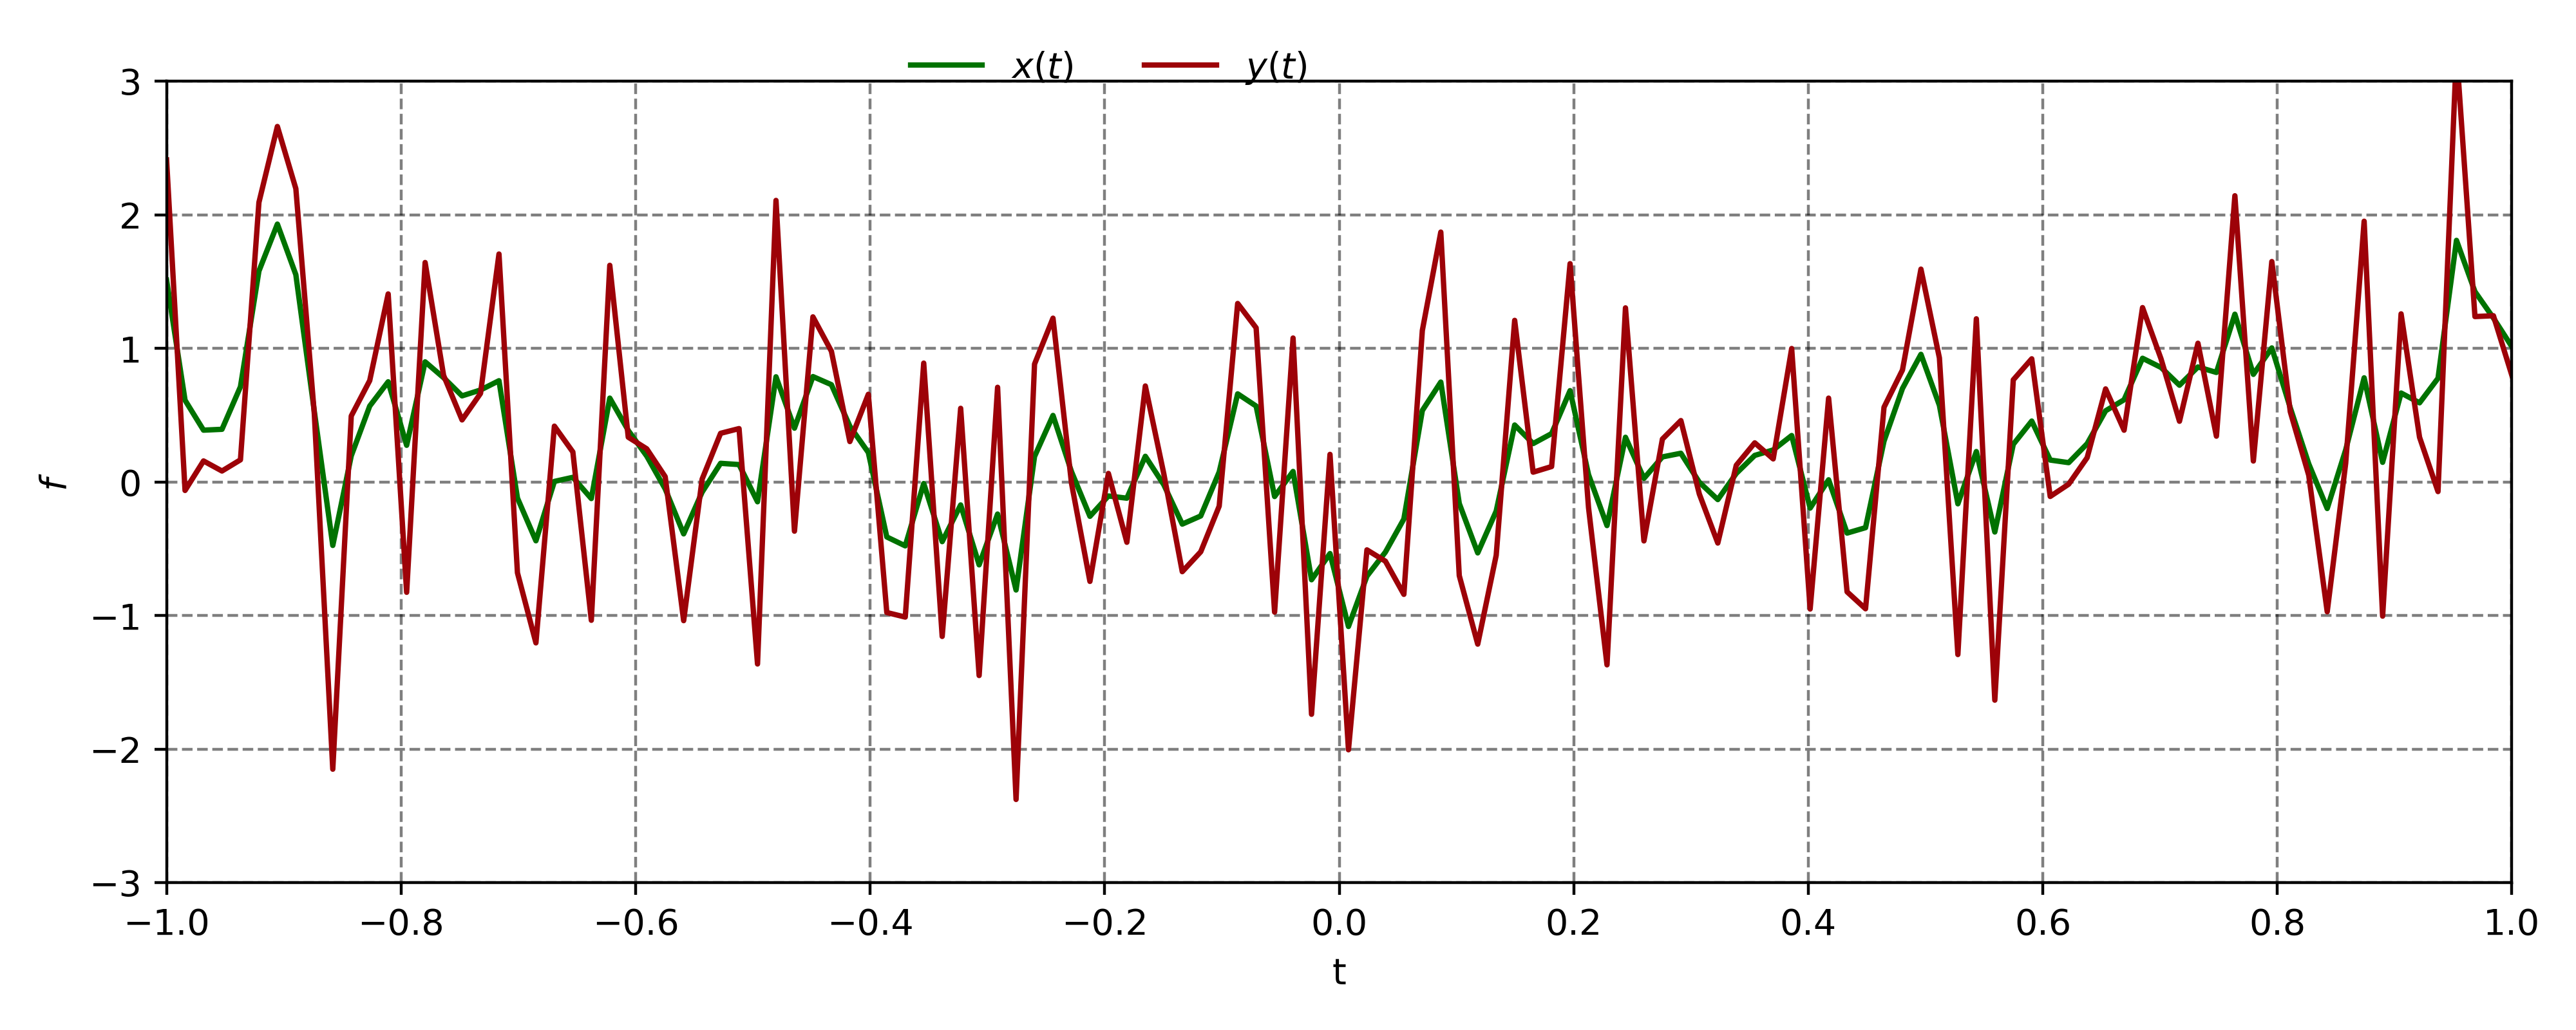
\includegraphics[width=12cm]{Graphics/Problema_3/lambda_1.png}
    \caption{Comparación de los valores de entrada ($y$) con los valores obtenidos $(x)$ al realizar el suavizado usando el método del descenso de gradiente.}
    \label{fig:lambda_1}
\end{figure}


\subsubsection{Segundo caso}

En la figura \ref{fig:lambda_10} se muestran los resultados de cada iteración obtenidos por la función de Rosembrock para el caso de $n=2$.

\begin{figure}[H]
    \centering
    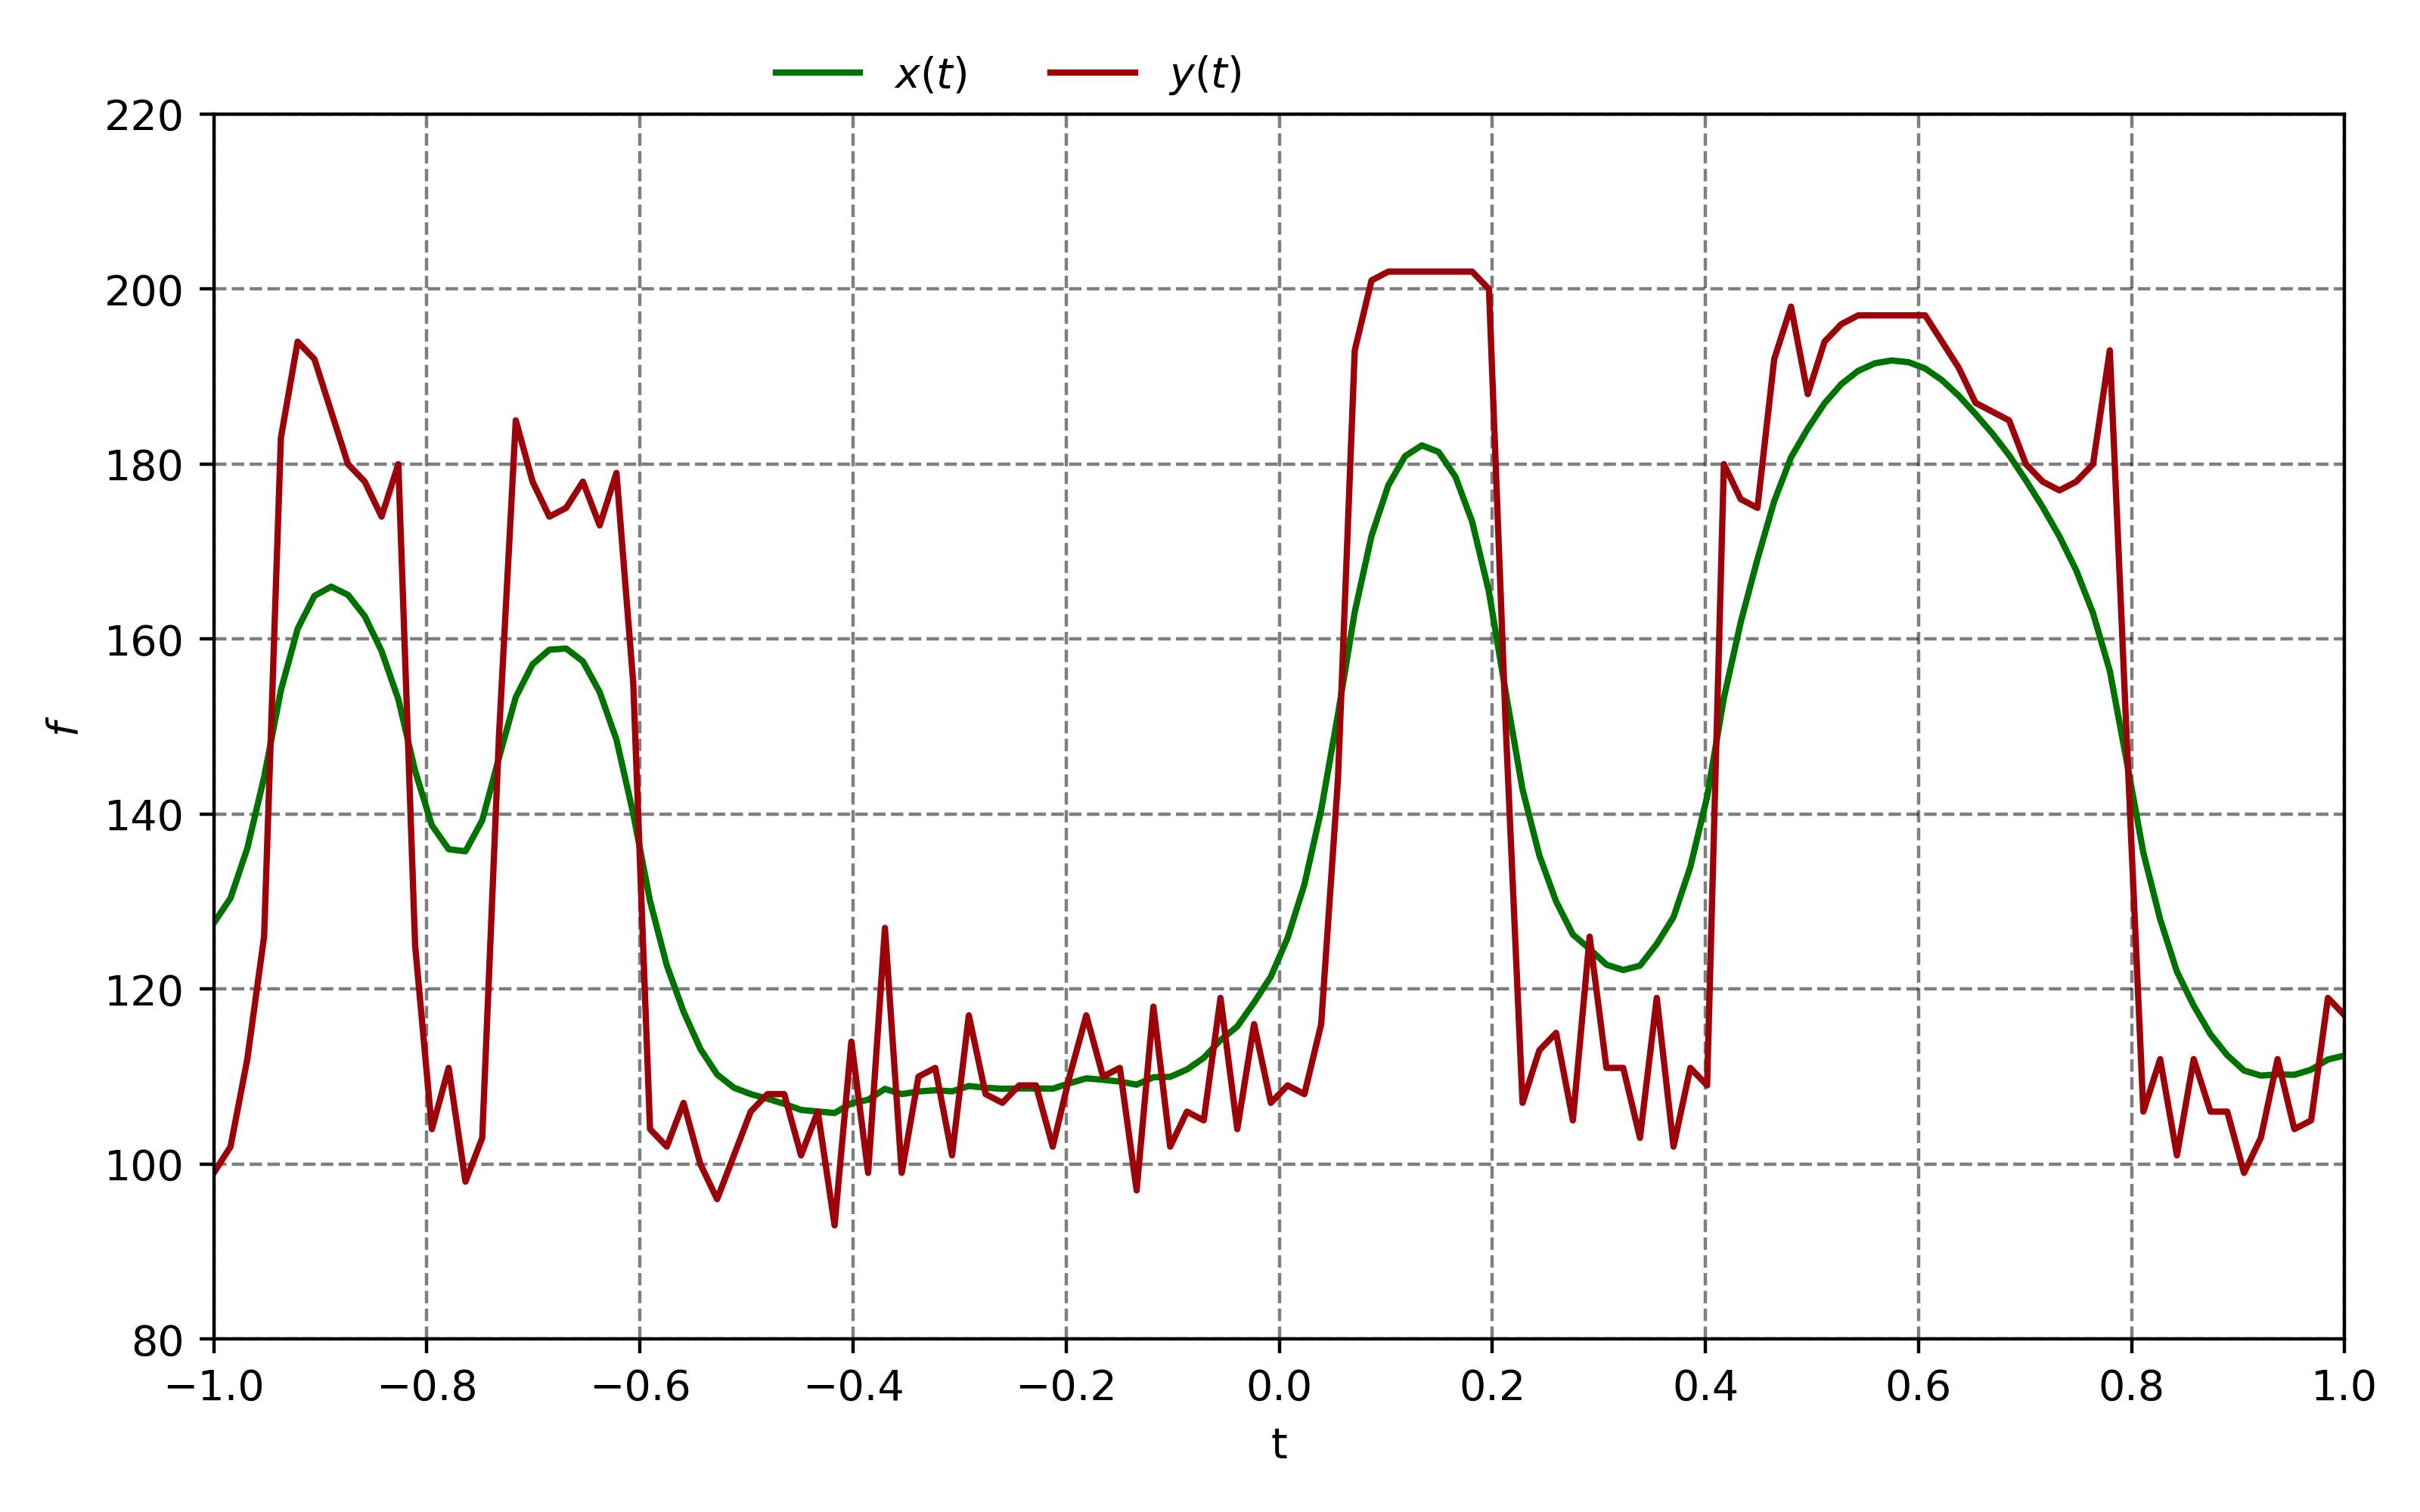
\includegraphics[width=12cm]{Graphics/Problema_3/lambda_10.png}
    \caption{Comparación de los valores de entrada ($y$) con los valores obtenidos $(x)$ al realizar el suavizado usando el método del descenso de gradiente.}
    \label{fig:lambda_10}
\end{figure}

\subsubsection{Tercer caso}

En la figura \ref{fig:lambda_1000} se muestran los resultados de cada iteración obtenidos por la función de Rosembrock para el caso de $n=2$.

\begin{figure}[H]
    \centering
    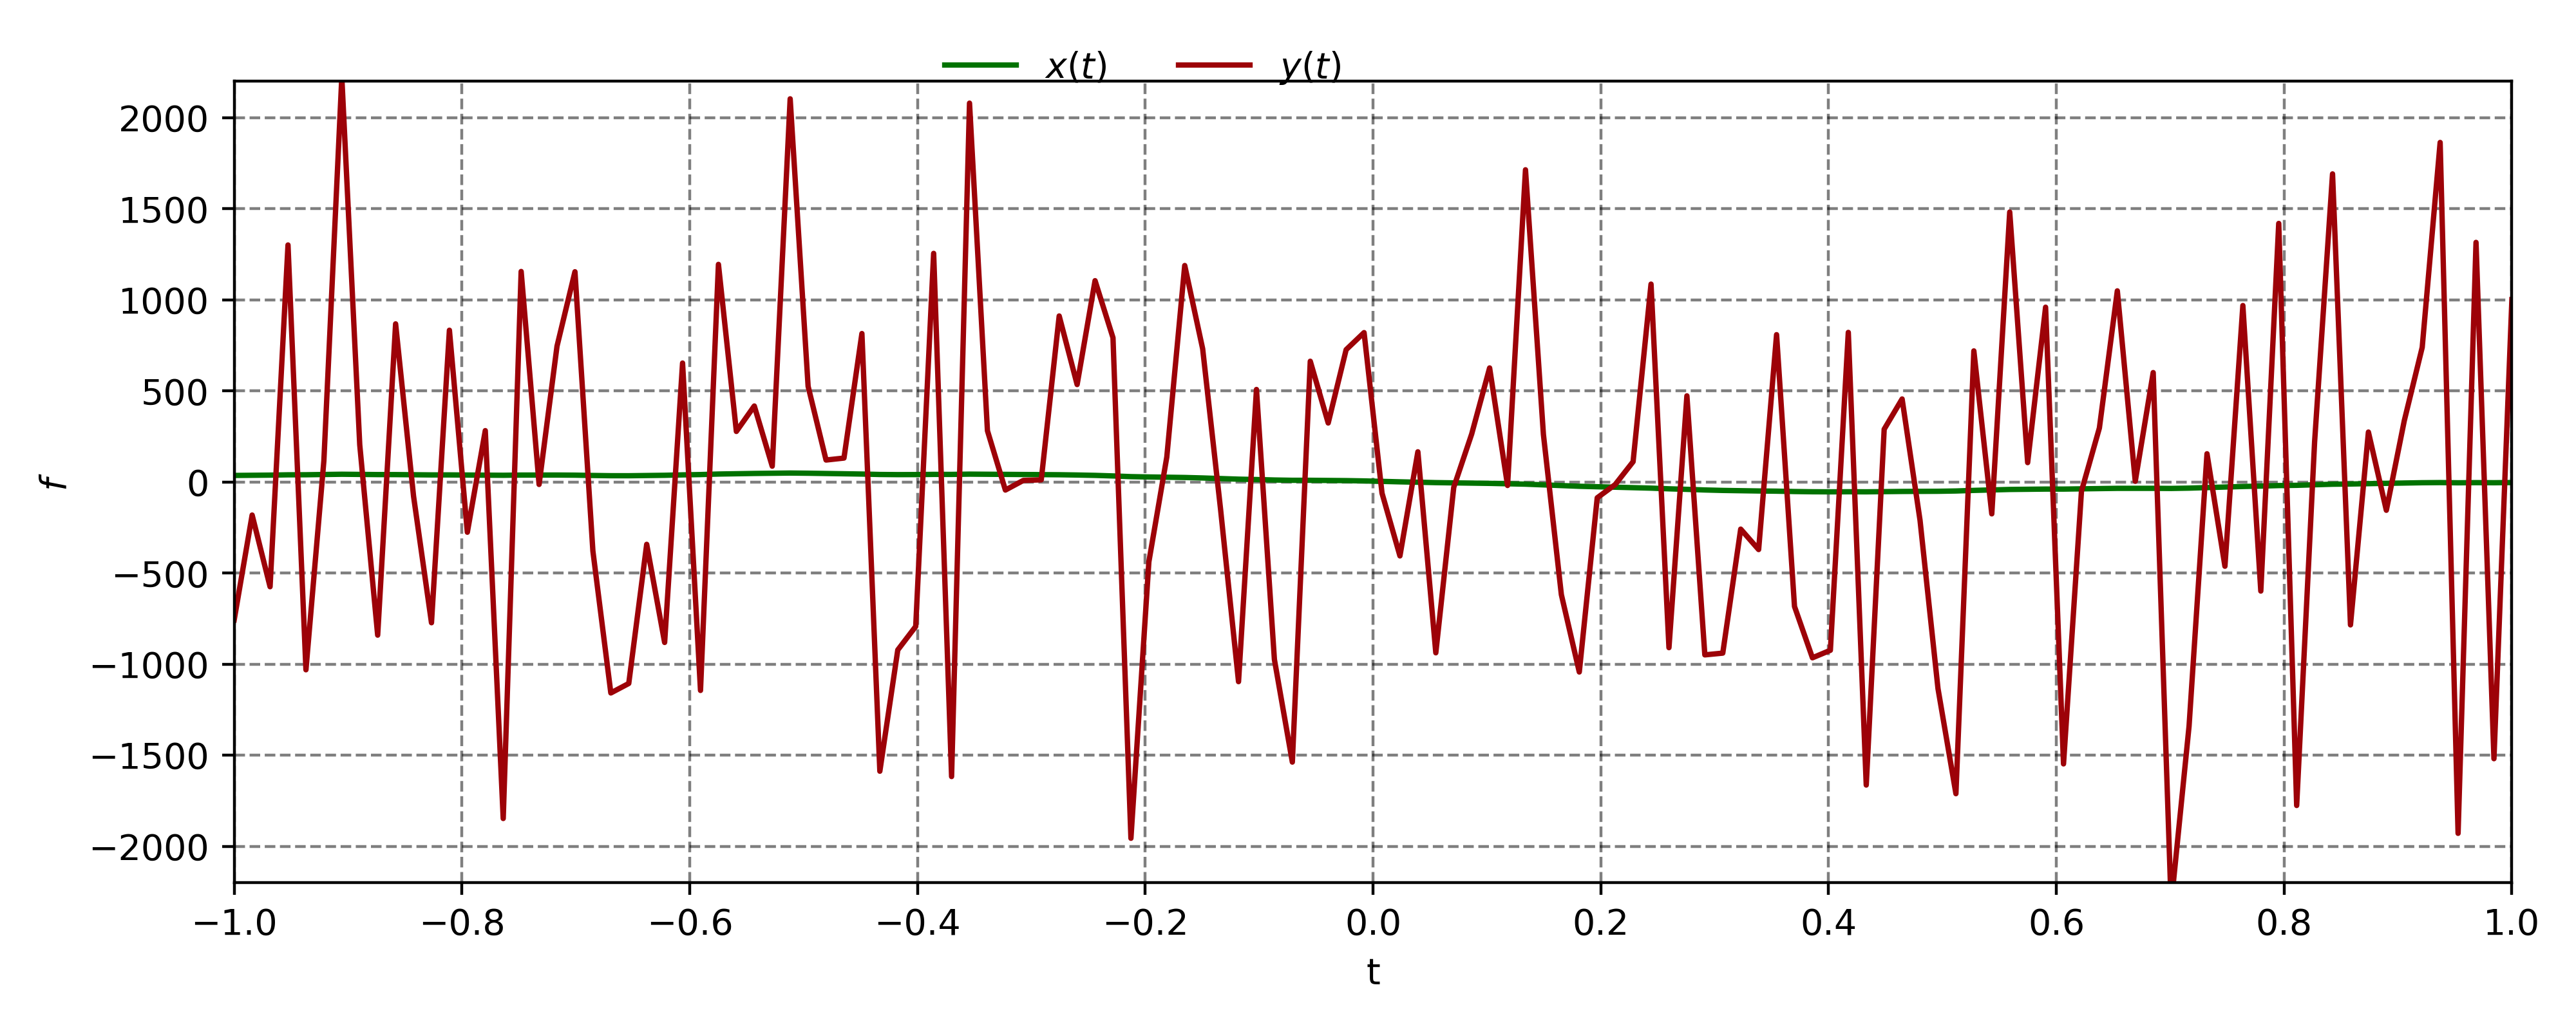
\includegraphics[width=12cm]{Graphics/Problema_3/lambda_1000.png}
    \caption{Comparación de los valores de entrada ($y$) con los valores obtenidos $(x)$ al realizar el suavizado usando el método del descenso de gradiente.}
    \label{fig:lambda_1000}
\end{figure}